
\chapter{Pohon}
\section{Představení systému}
Cílem práce je navrhnout řízení daného pohonu. Pohon se skládá z 5 fázového synchronního motoru s permanentními magenty. Blokové schéma elektrické části pohonu je na obrázku \ref{fig:elekticky blokac}.Ten je napájen 2 stupňovým střídačem. V práci uvažuji napájení střídače ideálním stejnosměrným napětím o velikosti $V_{DC}$. Daný pohon vychází z modelu pohonu v MATLAB.

\begin{figure}[h]
    \centering
    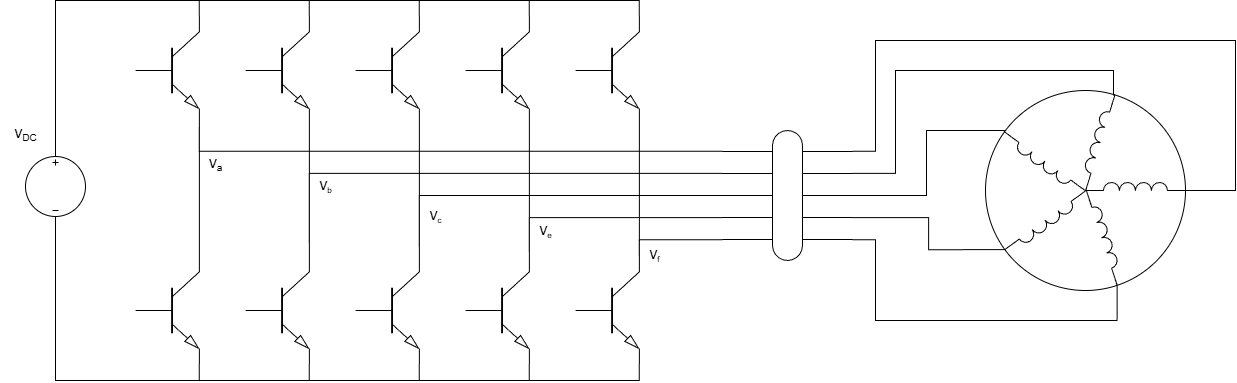
\includegraphics[width=\linewidth]{obrazky/electric.drawio.png}
    \caption{Blokové elektrické schéma pohonu}
    \label{fig:elekticky blokac}
\end{figure}

Blokové schéma řízení je na obrázku \ref{fig:block_control}. Řídící schéma má za cíl udržet požadované otáčky, a reagovat na primadonou změnu zátěže. Na motoru je možné měřit úhel jeho natočení, moment generovaný motorem a proud odebíraný motorem, ten odpovídá proudu statorem v práci označovaným jako $i_s$.

Měrné hodnoty jsou nejdřív transformovány do $dq$ souřadnic. Regulátor na jejich základě a generuje vektor požadovaného napětí $V_{\alpha \beta_{13}}^*$ v $dq$ souřadnicích. Modulátor následně generuje sekvenci přepnutí, kterou přímo ovládá střídač.



\begin{figure}[ht]
\centering
    \begin{tikzpicture}[
        x=\textwidth,
        block/.style={
            draw,
            rectangle,
            minimum height=1.2cm,
            minimum width=0.12\textwidth,
            align=center
        },
        arrow/.style={->, thick}
    ]
    % horní řada
    \node[block] (reg) {Regulátor};
    \node[block] (mod) [right=of reg] {Modulátor};
    \node[block] (inv) [right=of mod] {Střídač};
    \node[block] (mot) [right=of inv] {PMSM motor};
    % dolní řada
    \node[block] (dq) [below=of inv] {Transformace\\ $abcde \rightarrow dq_{13}$};
    
    % šipky
    \draw[arrow] (reg) -- node[above] {$\mathbf{V_{dq}}^*$} (mod);
    \draw[arrow] (mod) -- (inv);
    \draw[arrow] (inv) -- (mot);
    \draw[arrow] ([xshift=-1.5cm]reg.west) -- (reg.west) 
         node[above, pos=0.5, yshift=1mm] {$\mathbf{\omega_m^*}$};
         
    \draw[arrow] (dq.west)  -| (reg.south) 
         node[left, pos=0.5, yshift=1mm] {$ \mathbf{i_dq,T,\omega_m} $};
    
    
    
    % zalomená šipka od motoru k dq (pravý úhel)
    \draw[<-]  (dq.east) -| (mot.south) node[right, pos=00.5] {$\mathbf{i_{abc},T,\theta_m}$};
    \end{tikzpicture}
\caption{Blokové schéma řízení motoru}
\label{fig:block_control}
\end{figure}


